\chapter{Implementacija i korisničko sučelje}
		
		
		\section{Korištene tehnologije i alati}
		
%			\textbf{\textit{dio 2. revizije}}
			
% 			 \textit{Detaljno navesti sve tehnologije i alate koji su primijenjeni pri izradi dokumentacije i aplikacije. Ukratko ih opisati, te navesti njihovo značenje i mjesto primjene. Za svaki navedeni alat i tehnologiju je potrebno \textbf{navesti internet poveznicu} gdje se mogu preuzeti ili više saznati o njima}.
			
			
% 			\eject 
		
	        Komunikacija u teamu realizirana je korištenjem aplikacija Whatsapp i Discord. Organizacija rada i podjela na zadatke među članovima projekta ostvarene su pomoću  Microsoft SharePointa i Trello-a, a sastanci su održavani preko platvorme Microsoft Teams. Za izradu UML dijagrama korišten je alat Astah UML, za izradu grafova aplikacija Lucidchart, a kao sustav za upravljanje izvornim kodom Git. Udaljeni je repozitorij projekta dostupan na web platformi GitLab. Korištena je i platforma Heroku kao servisni oblak koji nudi razvoj web aplikacija i usluga. 
Kao razvojno okruženje korišten je IntelliJ IDEA Ultimate. To je višestruka platforma za Javu koja se može proširiti brojnim dodacima koji će ju učiniti još cjelovitijom. IntelliJ IDEA također pruža pomoć u kodiranju za širok spektar drugih jezika poput SQL-a, HTML-a i JavaScripta te predviđa potebe korisnika i automatizira zamorne i ponavljajuće zadatke kako bi mogao ostati fokusiran na širu sliku projekta.
Aplikacija je napisana koristeći radni okvir Spring Boot  u programskom jeziku Javi za izradu backenda ,React, skriptni programski jezik JavaScript, platforma Node.js, mrežni okvir s otvorenim kodom Bootstrap, prezentacijski jezik HTML te skriptni jezik CSS za izradu frontenda. Za izradu mapa korištena je aplikacija HERE WeGo. Upravljanje bazom podataka ostvarili smo pomoću sustava PostgreSQL. 
React, također poznat kao React.js ili ReactJS, je biblioteka u JavaScriptu za izgradnju korisničkih sučelja. Održavana je od strane Facebooka. React se najčešće koristi kao osnova u razvoju web ili mobilnih aplikacija. Složene aplikacije u Reactu obično zahtijevaju korištenje dodatnih biblioteka za interakciju s API-jem. Neke od karakteristika radnog okvira Spring Boot su: unaprijed pripremljene funkcionalnosti (eng. Out of the box functionalities), nema generiranja klasa i koda već se koriste unaprijed definirane biblioteke te set nefunkcionalnih alata i klasa u pogledu konfiguracije i pokretanja servera, sigurnosti, metrike te ostalih pomoćnih poslova.
\eject
		\section{Ispitivanje programskog rješenja}
% 			\textbf{\textit{dio 2. revizije}}\\
% 			 \textit{U ovom poglavlju je potrebno opisati provedbu ispitivanja implementiranih funkcionalnosti na razini komponenti i na razini cijelog sustava s prikazom odabranih ispitnih slučajeva. Studenti trebaju ispitati temeljnu funkcionalnost i rubne uvjete.}
\subsection{Ispitivanje komponenti}
% 			\textit{Potrebno je provesti ispitivanje jedinica (engl. unit testing) nad razredima koji implementiraju temeljne funkcionalnosti. Razraditi \textbf{minimalno 6 ispitnih slučajeva} u kojima će se ispitati redovni slučajevi, rubni uvjeti te izazivanje pogreške (engl. exception throwing). Poželjno je stvoriti i ispitni slučaj koji koristi funkcionalnosti koje nisu implementirane. Potrebno je priložiti izvorni kôd svih ispitnih slučajeva te prikaz rezultata izvođenja ispita u razvojnom okruženju (prolaz/pad ispita). }
			\begin{figure}[H] 					\centering 				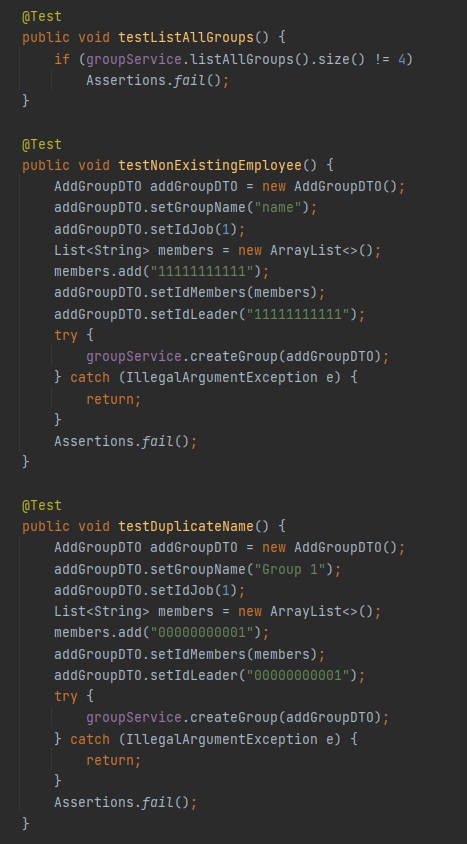
\includegraphics[height=0.7\textheight]{Dokumentacija/ispit-komp/GroupServiceTest 1.png}
				\caption{GroupServiceTest 1. dio}
				\end{figure}
                \begin{figure}[H] 					\centering 					                    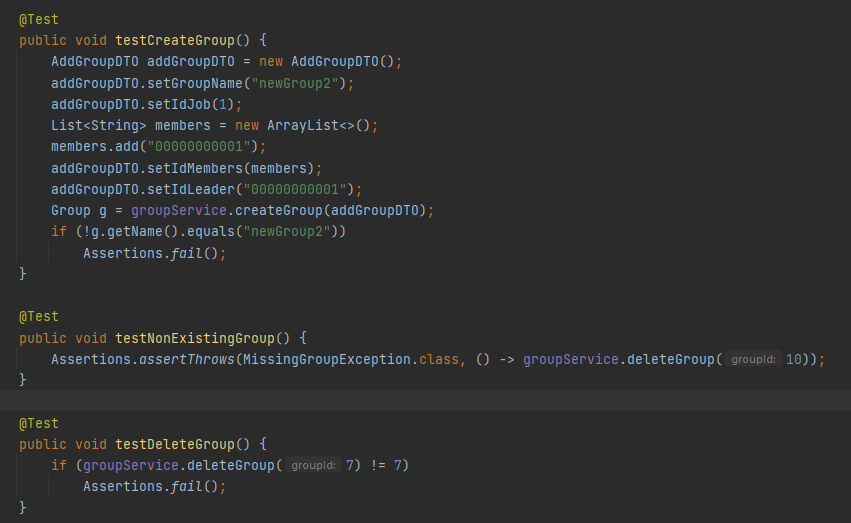
\includegraphics[width=\textwidth,height=\textheight,keepaspectratio]{Dokumentacija/ispit-komp/GroupServiceTest2.png}
				\caption{GroupServiceTest 2. dio}
				\end{figure}
				\begin{figure}[H] 					\centering 					                    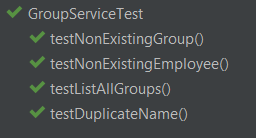
\includegraphics[width=\textwidth]{Dokumentacija/ispit-komp/GroupServiceTestRez. dio.png}
				\caption{GroupServiceTest rezultati 1. dio}
				\end{figure}
				\begin{figure}[H] 					\centering 					                    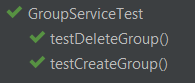
\includegraphics[width=\textwidth]{Dokumentacija/ispit-komp/GroupServiceTestRez2.png}
				\caption{GroupServiceTest rezultati 2. dio}
				\end{figure}
				
				
				
				\begin{figure}[H] 					\centering 				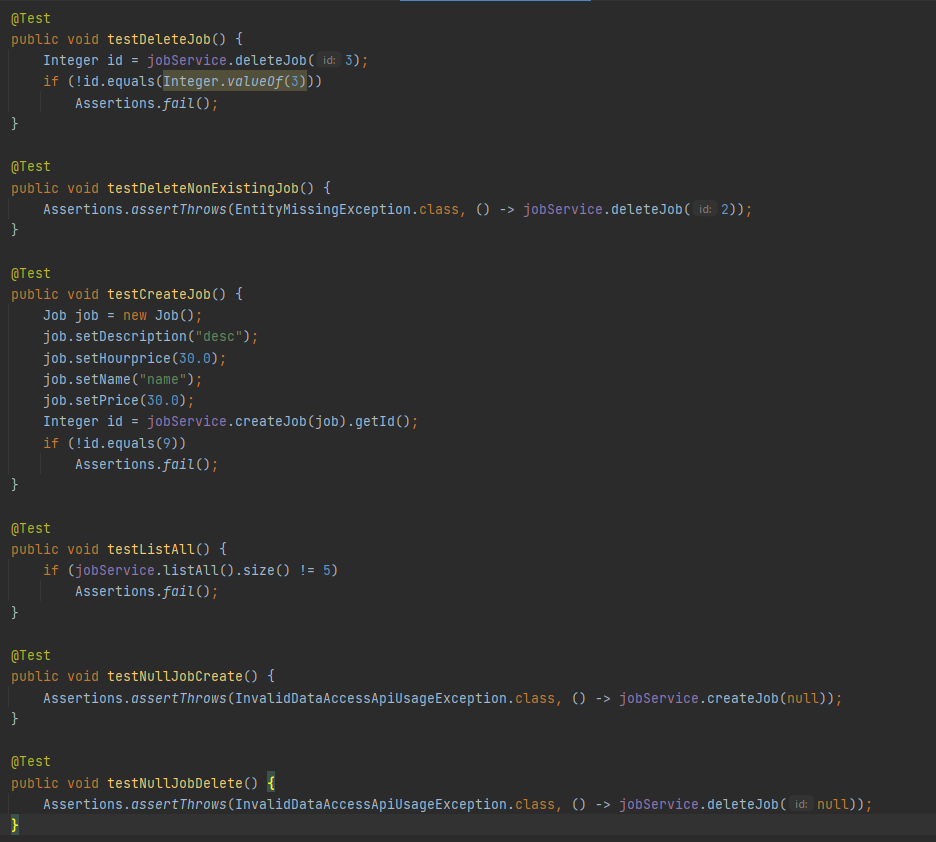
\includegraphics[width=\textwidth]{Dokumentacija/ispit-komp/JobServiceTest.png}
				\caption{JobServiceTest}
				\end{figure}
                \begin{figure}[H] 					\centering 					                    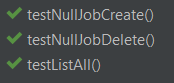
\includegraphics[width=\textwidth,height=\textheight,keepaspectratio]{Dokumentacija/ispit-komp/JobServiceTest - rezultati 1. dio.png}
				\caption{JobServiceTest rezultati 1. dio}
				\end{figure}
				\begin{figure}[H] 					\centering 					                    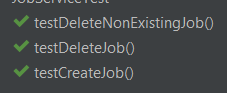
\includegraphics[width=\textwidth]{Dokumentacija/ispit-komp/JobServiceTest - rezultati 2. dio.png}
				\caption{JobServiceTest rezultati 2. dio}
				\end{figure}
				\eject
				
				
				
				\begin{figure}[H] 					\centering 				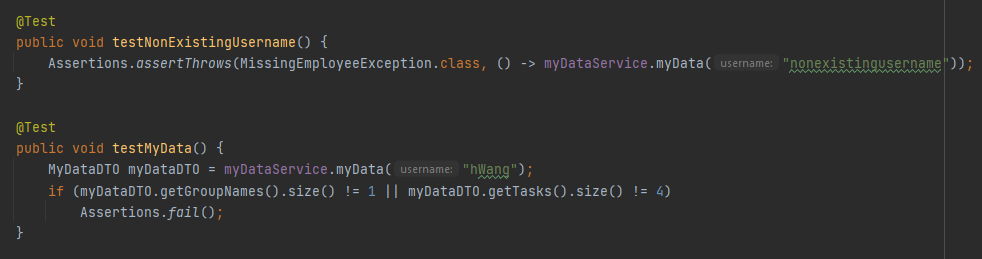
\includegraphics[width=\textwidth]{Dokumentacija/ispit-komp/MyDataServiceTest.png}
				\caption{MyDataServiceTest}
				\end{figure}
                \begin{figure}[H] 					\centering 					                    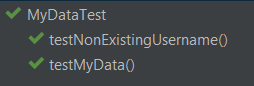
\includegraphics[width=\textwidth]{Dokumentacija/ispit-komp/MyDataServiceTest - rezultati.png}
				\caption{MyDataServiceTest rezultati}
				\end{figure}
				
				
				\begin{figure}[H] 					\centering 				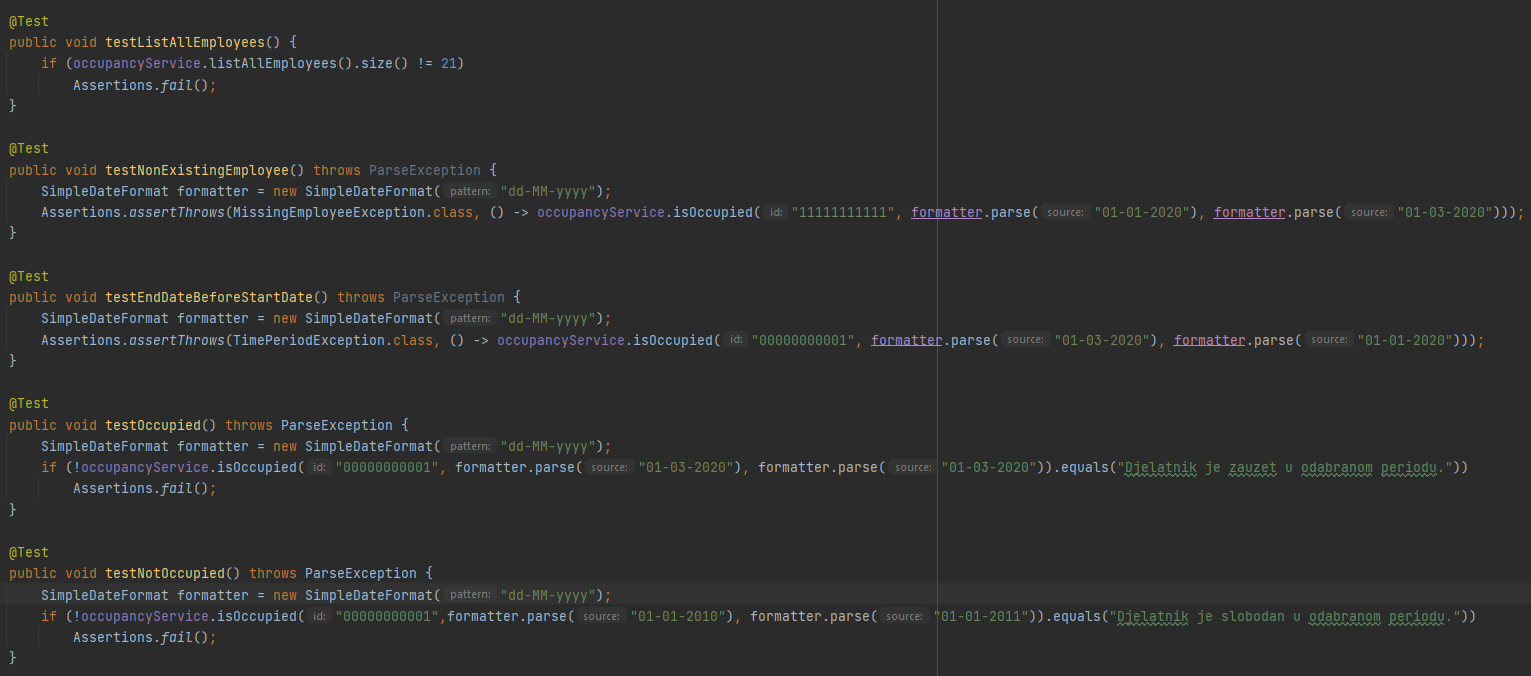
\includegraphics[width=\textwidth]{Dokumentacija/ispit-komp/OccupancyServiceTest.png}
				\caption{OccupancyServiceTest}
				\end{figure}
                \begin{figure}[H] 					\centering 					                    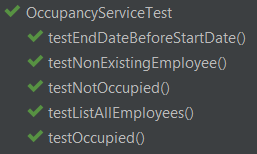
\includegraphics[width=\textwidth]{Dokumentacija/ispit-komp/OccupancyServiceTest - rezultati.png}
				\caption{OccupancyServiceTest rezultati}
				\end{figure}
				
				
				
				\begin{figure}[H] 					\centering 				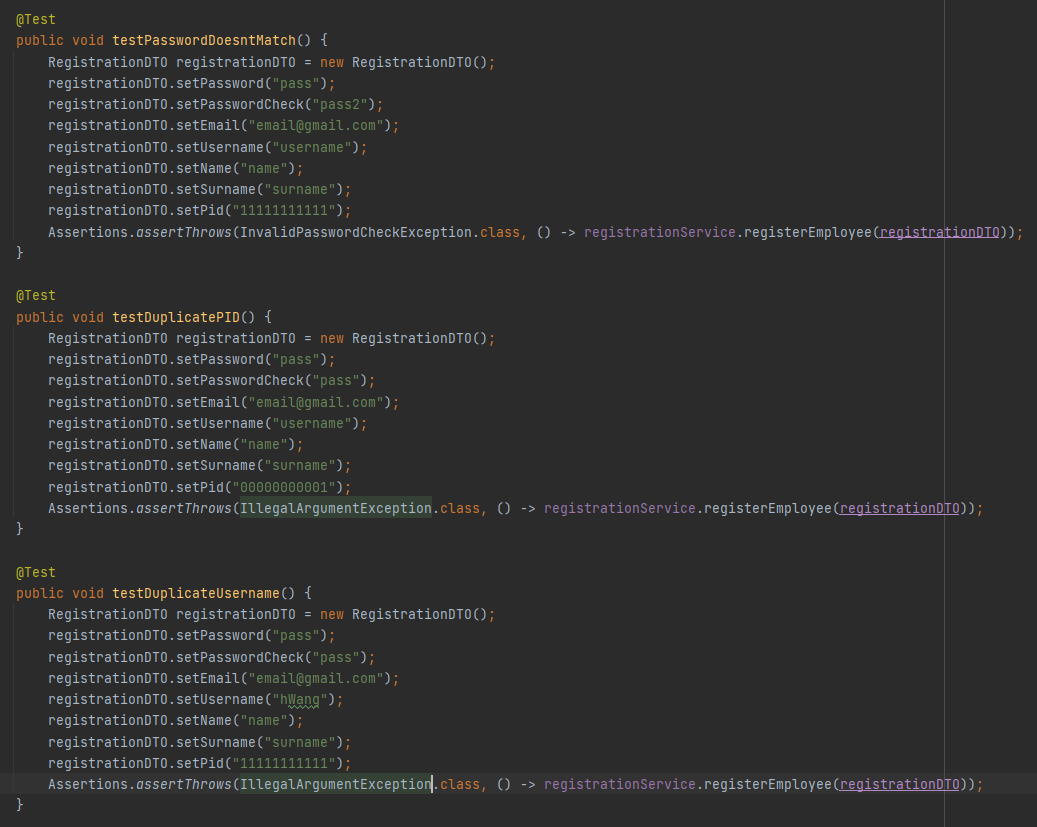
\includegraphics[width=\textwidth]{Dokumentacija/ispit-komp/RegistrationServiceTest - 1. dio.png}
				\caption{RegistrationServiceTest}
				\end{figure}
                \begin{figure}[H] 					\centering 					                    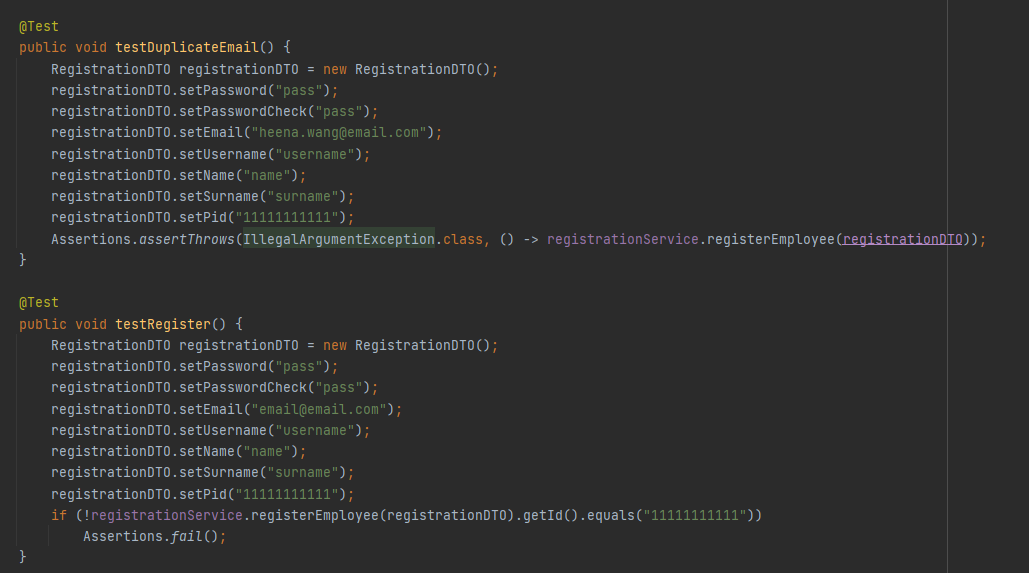
\includegraphics[width=\textwidth]{Dokumentacija/ispit-komp/RegistrationServiceTest - 2. dio.png}
				\caption{RegistrationServiceTest rezultati 1. dio}
				\end{figure}
				\begin{figure}[H] 					\centering 					                    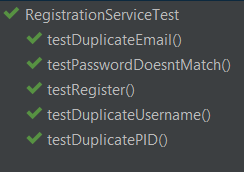
\includegraphics[width=\textwidth]{Dokumentacija/ispit-komp/RegistrationServiceTest - rezultati.png}
				\caption{RegistrationServiceTest rezultati 2. dio}
				\end{figure}
				
				
				\begin{figure}[H] 					\centering 				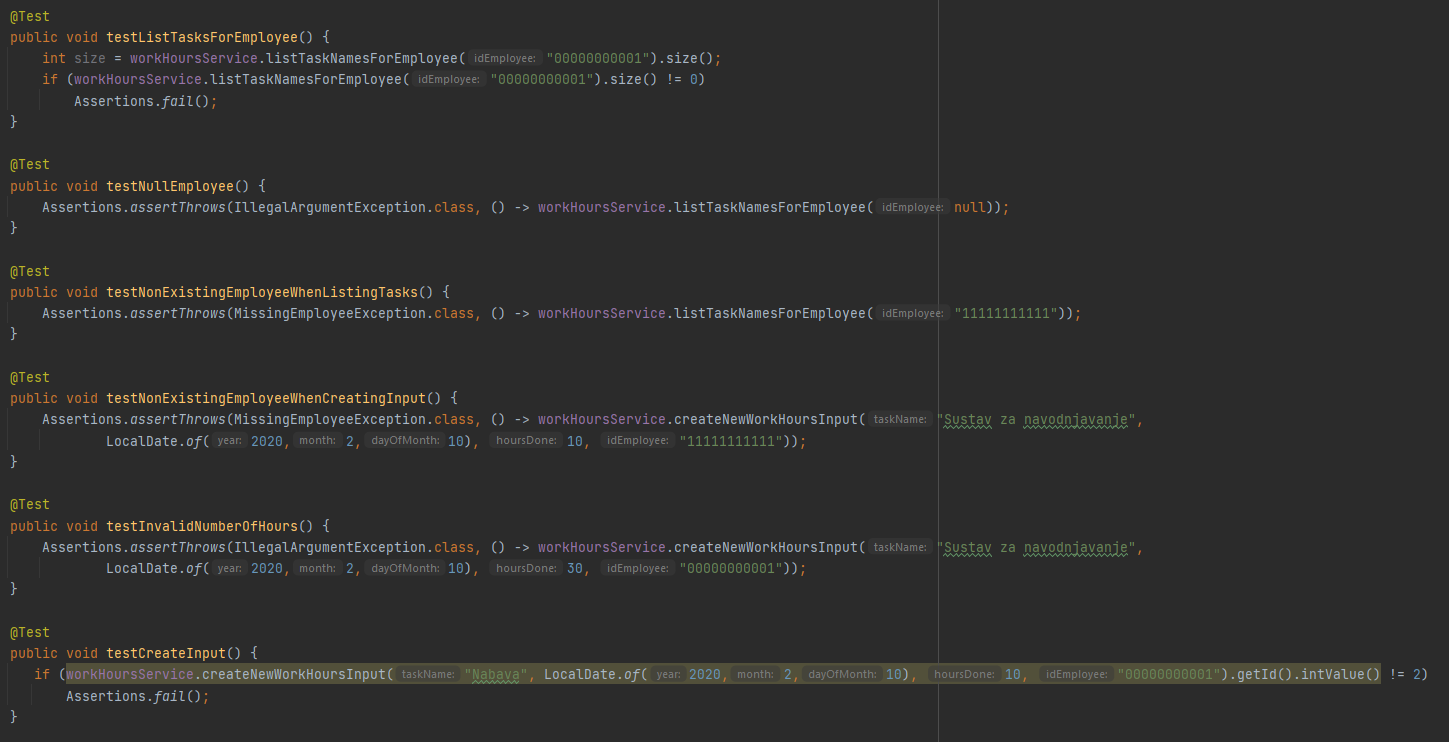
\includegraphics[width=\textwidth]{Dokumentacija/ispit-komp/WorkHoursServiceTest.png}
				\caption{WorkHoursServiceTest}
				\end{figure}
                \begin{figure}[H] 					\centering 					                    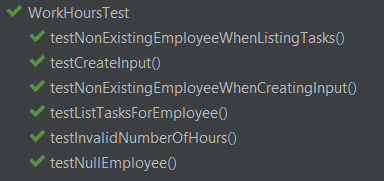
\includegraphics[width=\textwidth]{Dokumentacija/ispit-komp/WorkHoursServiceTest - rezultati.png}
				\caption{WorkHoursServiceTest rezultati}
				\end{figure}
				
				\begin{figure}[H] 					\centering 				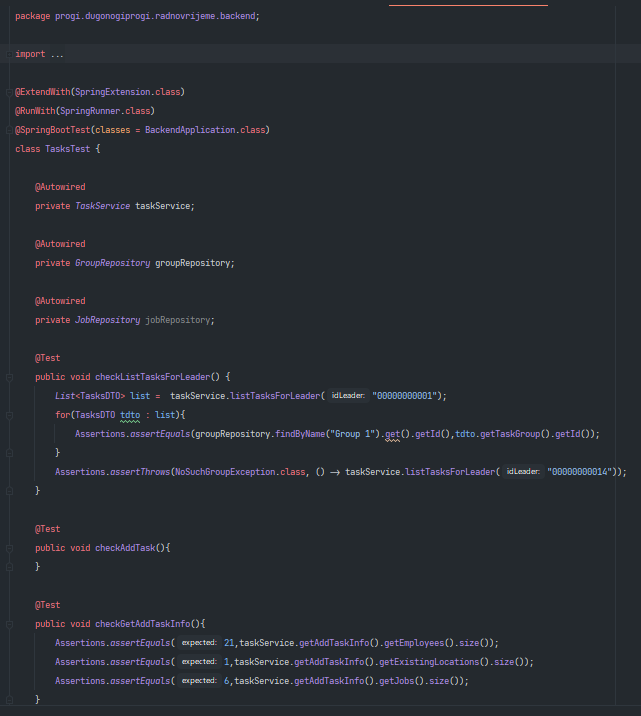
\includegraphics[width=\textwidth]{Dokumentacija/ispit-komp/Taskstest.png}
				\caption{TasksServiceTest}
				\end{figure}
                \begin{figure}[H] 					\centering 					                    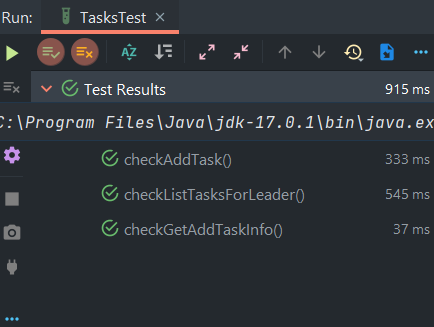
\includegraphics[width=\textwidth]{Dokumentacija/ispit-komp/TaskTestResult.png}
				\caption{TasksServiceTest rezultati}
				\end{figure}
				
				\begin{figure}[H] 					\centering 				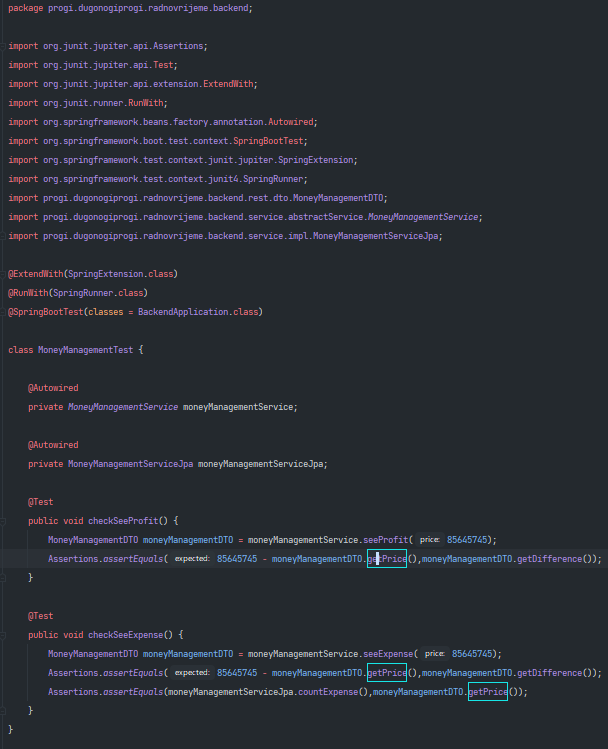
\includegraphics[width=\textwidth]{Dokumentacija/ispit-komp/MoneyManagementtest.png}
				\caption{MoneyManagementServiceTest}
				\end{figure}
                \begin{figure}[H] 					\centering 					                    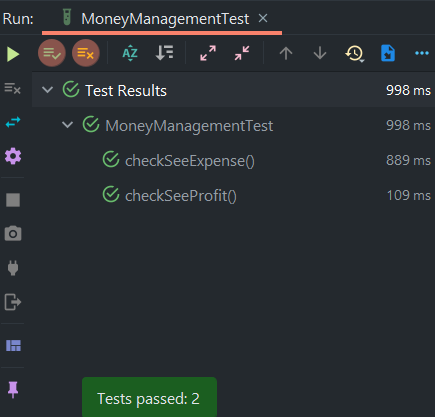
\includegraphics[width=\textwidth]{Dokumentacija/ispit-komp/MoneyManagementResult.png}
				\caption{MoneyManagementServiceTest rezultati}
				\end{figure}
				
				\begin{figure}[H] 					\centering 				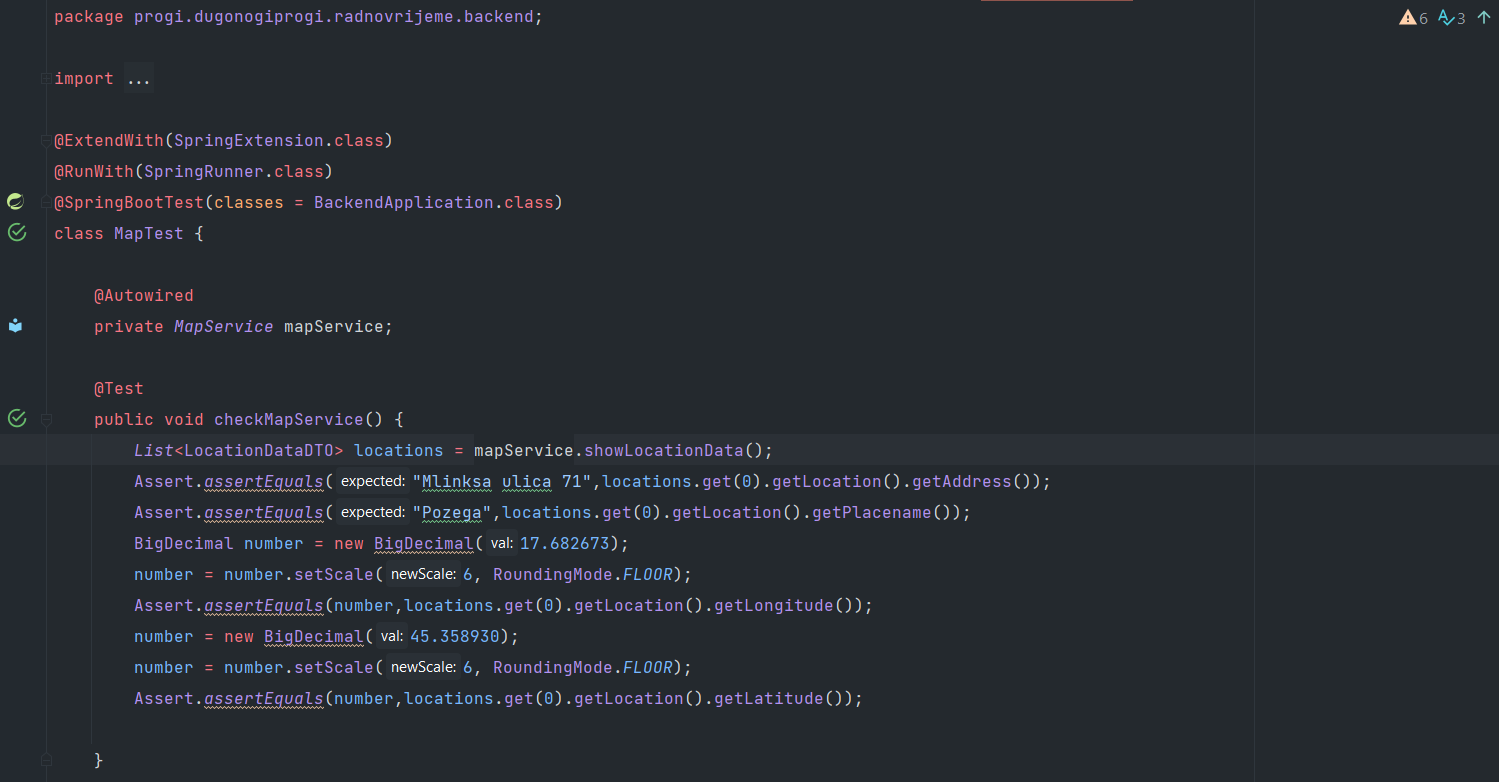
\includegraphics[width=\textwidth]{Dokumentacija/ispit-komp/mapTest.png}
				\caption{MapServiceTest}
				\end{figure}
                \begin{figure}[H] 					\centering 					                    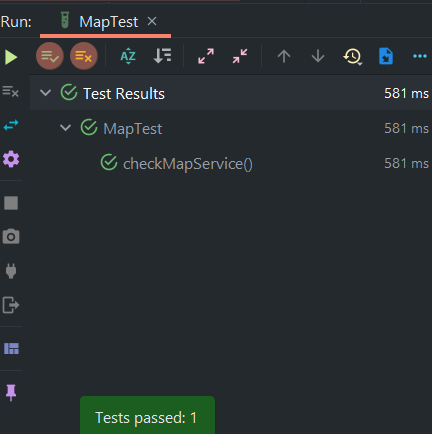
\includegraphics[width=\textwidth]{Dokumentacija/ispit-komp/mapTestResult.png}
				\caption{MapServiceTest rezultati}
				\end{figure}
				
                
			
			\eject 			
			
			
			
			\subsection{Ispitivanje sustava}
			
			 %\textit{Potrebno je provesti i opisati ispitivanje sustava koristeći radni okvir Selenium\footnote{\url{https://www.seleniumhq.org/}}. Razraditi \textbf{minimalno 4 ispitna slučaja} u kojima će se ispitati redovni slučajevi, rubni uvjeti te poziv funkcionalnosti koja nije implementirana/izaziva pogrešku kako bi se vidjelo na koji način sustav reagira kada nešto nije u potpunosti ostvareno. Ispitni slučaj se treba sastojati od ulaza (npr. korisničko ime i lozinka), očekivanog izlaza ili rezultata, koraka ispitivanja i dobivenog izlaza ili rezultata.\\ }
			 
			 %\textit{Izradu ispitnih slučajeva pomoću radnog okvira Selenium moguće je provesti pomoću jednog od sljedeća dva alata:}
			 %\begin{itemize}
			 %	\item \textit{dodatak za preglednik \textbf{Selenium IDE} - snimanje korisnikovih akcija radi automatskog ponavljanja ispita	}
			 %	\item \textit{\textbf{Selenium WebDriver} - podrška za pisanje ispita u jezicima Java, C\#, PHP koristeći posebno programsko sučelje.}
			 %\end{itemize}
		 	% \textit{Detalji o korištenju alata Selenium bit će prikazani na posebnom predavanju tijekom semestra.}
		 	    
		 	 

Ispitni slučaj 1: \textbf{Prijava vlasnika} 


\begin{itemize}
 	\item \textit{ \textbf{Ulaz: }korisničko ime: cTalley, lozinka: pass}
 	\item \textit{\textbf{Očekivani izlaz: }uspješna prijava i preusmjeravanje na početnu stranicu, navigacijska traka prikazuje stranice dostupne vlasniku }
 	\item \textit{\textbf{Dobiveni izlaz: }uspješna prijava i preusmjeravanje na početnu stranicu, navigacijska traka prikazuje stranice dostupne vlasniku }
 	\item \textit{\textbf{Rezultat ispitivanja: }uspješno}
 \end{itemize}
 \begin{figure}[H] 					\centering 					\includegraphics[width=\textwidth]{Picture1}
				\caption{Selenium test 1}
				\end{figure}
\begin{figure}[H] 					\centering 					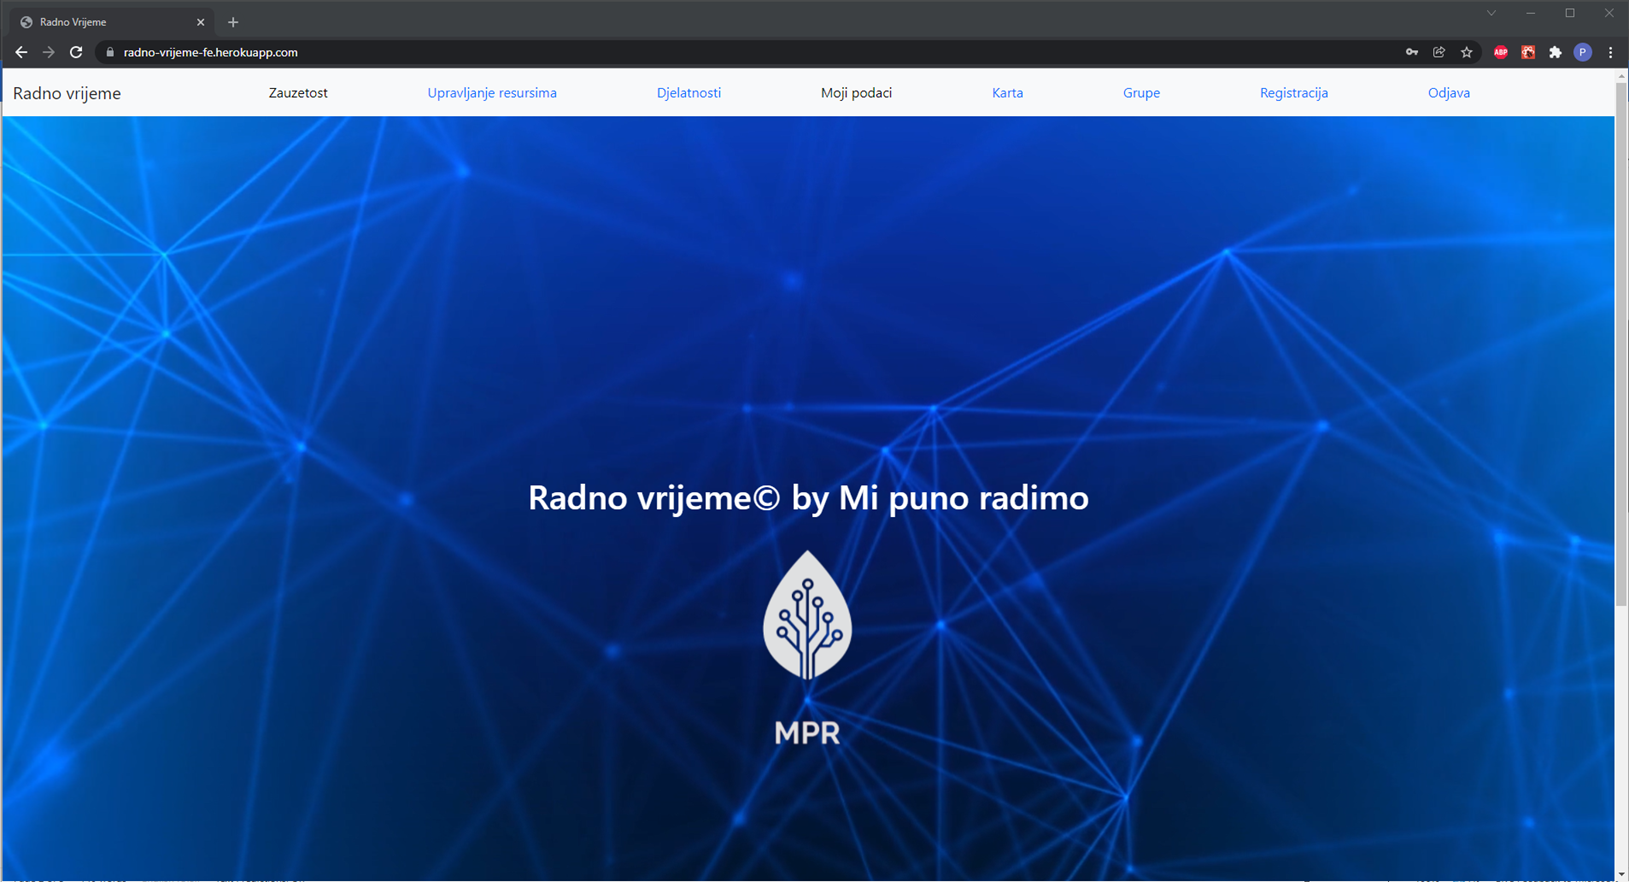
\includegraphics[width=\textwidth]{Picture2}
				\caption{Rezultat 1}
				\end{figure}
\eject
 
Ispitni slučaj 2: \textbf{Prijava vođe tima} 


\begin{itemize}
 	\item \textit{ \textbf{Ulaz: }korisničko ime: hWang, lozinka: pass }
 	\item \textit{\textbf{Očekivani izlaz: }uspješna prijava i preusmjeravanje na početnu stranicu, navigacijska traka prikazuje stranice dostupne vođi tima }
 	\item \textit{\textbf{Dobiveni izlaz: }uspješna prijava i preusmjeravanje na početnu stranicu, navigacijska traka prikazuje stranice dostupne vođi tima }
 	\item \textit{\textbf{Rezultat ispitivanja: }uspješno}
 \end{itemize}
                \begin{figure}[H] 					\centering 					                \includegraphics[width=\textwidth]{Picture3}
				\caption{Selenium test 2}
				\end{figure}
			    \begin{figure}[H] 					\centering 					\includegraphics[width=\textwidth]{Picture4}
				\caption{Rezultat 2}
				\end{figure}
%\eject 
  
Ispitni slučaj 3: \textbf{Prijava zaposlenika } 


\begin{itemize}
 	\item \textit{ \textbf{Ulaz: }korisničko ime: aBevan, lozinka: pass}
 	\item \textit{\textbf{Očekivani izlaz: }uspješna prijava i preusmjeravanje na početnu stranicu, navigacijska traka prikazuje stranice dostupne zaposleniku}
 	\item \textit{\textbf{Dobiveni izlaz: }uspješna prijava i preusmjeravanje na početnu stranicu, navigacijska traka prikazuje stranice dostupne zaposleniku }
 	\item \textit{\textbf{Rezultat ispitivanja: }uspješno}
 \end{itemize}
                \begin{figure}[H] 					\centering 					                \includegraphics[width=\textwidth]{Picture5}
				\caption{Selenium test 3}
				\end{figure}
			    \begin{figure}[H] 					\centering 					\includegraphics[width=\textwidth]{Picture6}
				\caption{Rezultat 3}
				\end{figure}
\eject

Ispitni slučaj 4: \textbf{Prijava nepostojećeg korisnika} 


\begin{itemize}
 	\item \textit{ \textbf{Ulaz: }korisničko ime: nekiKorisnik, lozinka: pass}
 	\item \textit{\textbf{Očekivani izlaz: }poruka o neuspješnoj prijavi }
 	\item \textit{\textbf{Dobiveni izlaz: }poruka o neuspješnoj prijavi }
 	\item \textit{\textbf{Rezultat ispitivanja: }uspješno}
 \end{itemize}
                \begin{figure}[H] 					\centering 					                \includegraphics[width=\textwidth]{Picture7}
				\caption{Selenium test 4}
				\end{figure}
			    \begin{figure}[H] 					\centering 					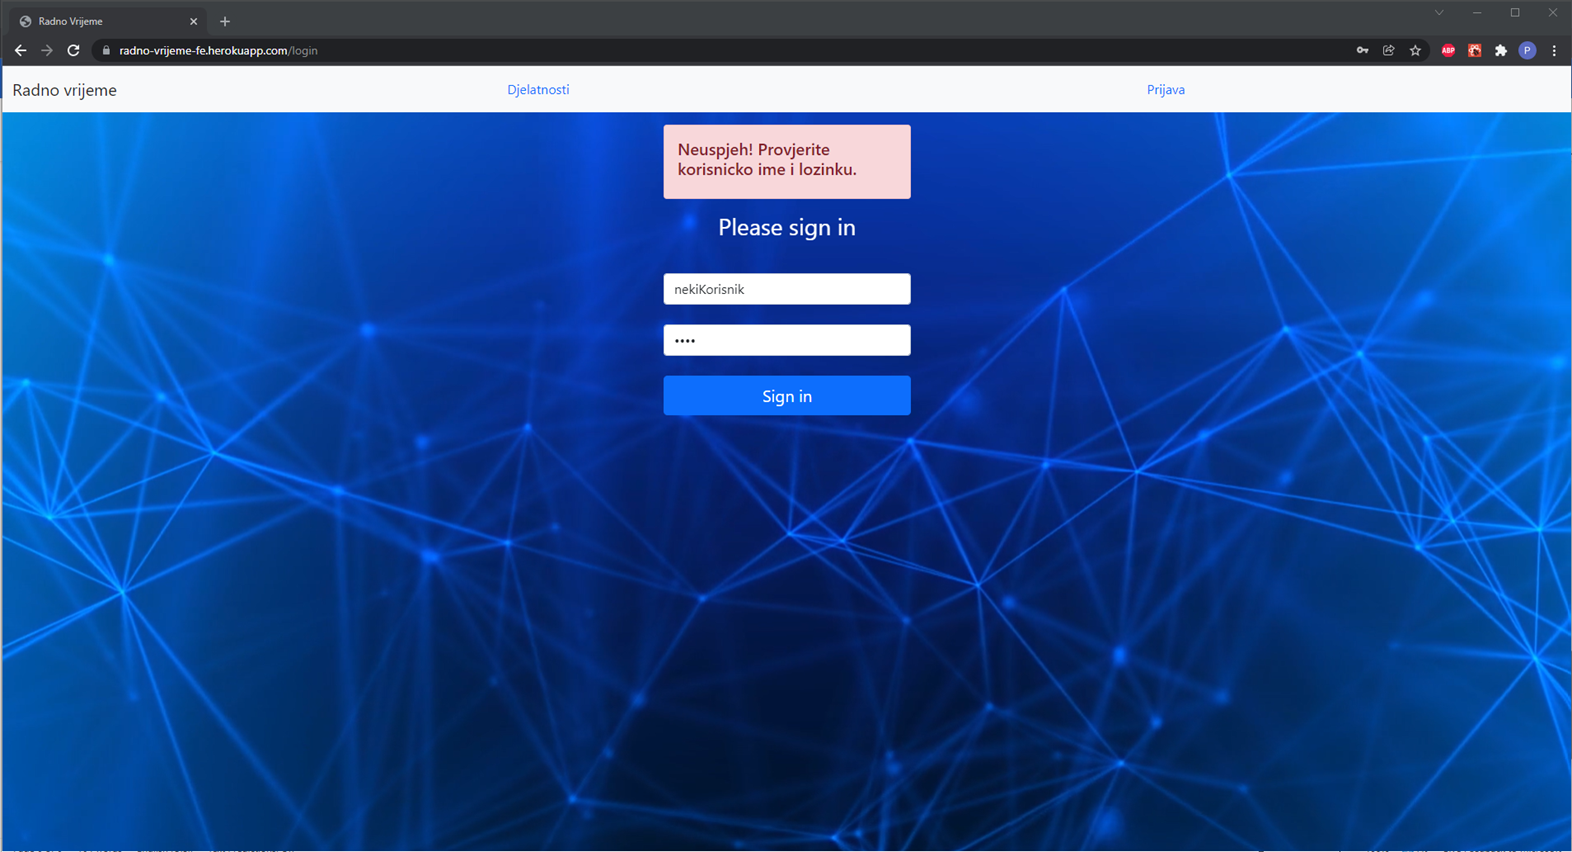
\includegraphics[width=\textwidth]{Picture8}
				\caption{Rezultat 4}
				\end{figure}
\eject 
		
		
		\section{Dijagram razmještaja}
			
% 			\textbf{\textit{dio 2. revizije}}
			
% 			 \textit{Potrebno je umetnuti \textbf{specifikacijski} dijagram razmještaja i opisati ga. Moguće je umjesto specifikacijskog dijagrama razmještaja umetnuti dijagram razmještaja instanci, pod uvjetom da taj dijagram bolje opisuje neki važniji dio sustava.}
Dijagram razreda prikazuje izvršnu arhitekturu sustava. Sustav je baziran na arhitekturi REST koja odvaja klijente od servera. Pomoću web preglednika, klijenti pristupaju poslužitelju fontend dijela naše aplikacije. Ta komunikacija odvija se putem HTTP veze. Poslužitelj frontend dijela zatim dohvaća podatke u JSON formatu sa back-end poslužitelja također putem HTTP veze. Frontend i backend aplikacije, iako odvojene, obje se nalaze na Heroku poslužitelju. Backend poslužitelj u izravnoj je komunikaciji s poslužiteljem baze podataka koja se nalazi na Amazon WS poslužitelju. 

\begin{figure}[H] 					\centering 					                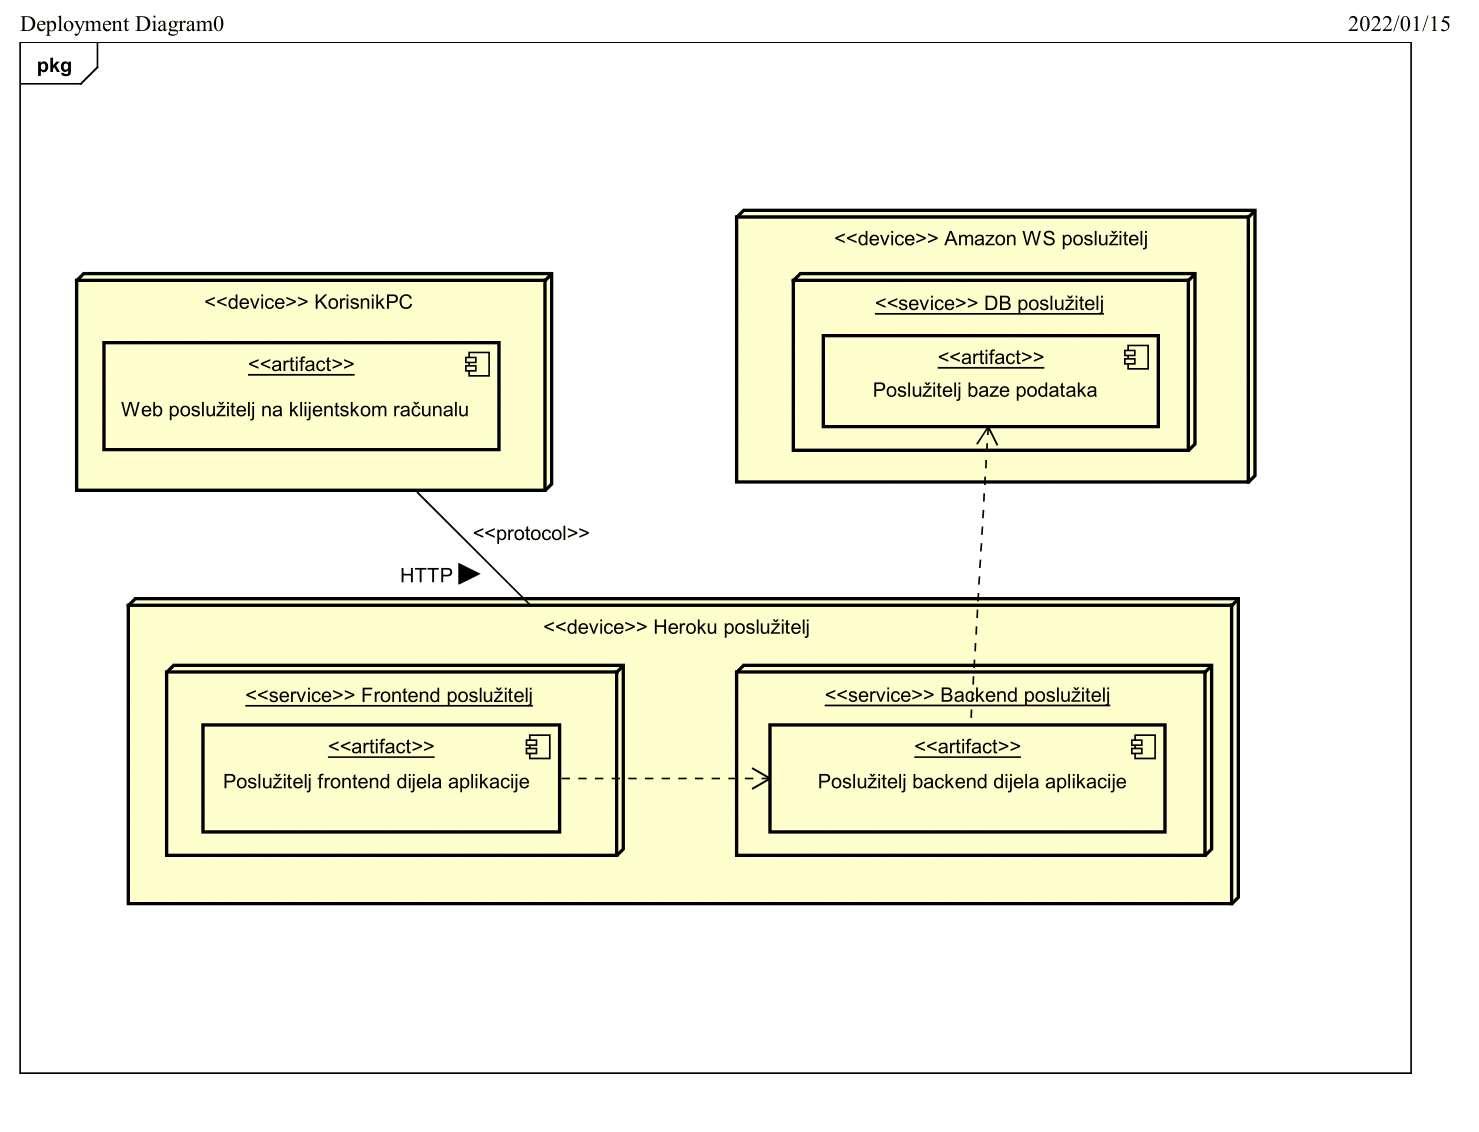
\includegraphics[width=\textwidth]{diagrazm}
				\caption{Dijagram razmještaja}
				\end{figure}


			
			\eject 
		
		\section{Upute za puštanje u pogon}
		
% 			\textbf{\textit{dio 2. revizije}}\\
		
% 			 \textit{U ovom poglavlju potrebno je dati upute za puštanje u pogon (engl. deployment) ostvarene aplikacije. Na primjer, za web aplikacije, opisati postupak kojim se od izvornog kôda dolazi do potpuno postavljene baze podataka i poslužitelja koji odgovara na upite korisnika. Za mobilnu aplikaciju, postupak kojim se aplikacija izgradi, te postavi na neku od trgovina. Za stolnu (engl. desktop) aplikaciju, postupak kojim se aplikacija instalira na računalo. Ukoliko mobilne i stolne aplikacije komuniciraju s poslužiteljem i/ili bazom podataka, opisati i postupak njihovog postavljanja. Pri izradi uputa preporučuje se \textbf{naglasiti korake instalacije uporabom natuknica} te koristiti što je više moguće \textbf{slike ekrana} (engl. screenshots) kako bi upute bile jasne i jednostavne za slijediti.}
			
			
% 			 \textit{Dovršenu aplikaciju potrebno je pokrenuti na javno dostupnom poslužitelju. Studentima se preporuča korištenje neke od sljedećih besplatnih usluga: \href{https://aws.amazon.com/}{Amazon AWS}, \href{https://azure.microsoft.com/en-us/}{Microsoft Azure} ili \href{https://www.heroku.com/}{Heroku}. Mobilne aplikacije trebaju biti objavljene na F-Droid, Google Play ili Amazon App trgovini.}
\textbf{Priprema alata za puštanje aplikacija u pogon na Heroku}

    Potrebno je instalirati Git i Heroku CLI pomoću windows installera koji se može jednostavno naći na internetu na njihovim službenim stranicama. Također treba napraviti korisnički račun na Heroku. Nakon što je to postavljeno potrebno je skinuti Repozitorij \textit{radno\char`_vrijeme}. 
    
\textbf{Puštanje backend aplikacije u pogon} 

Prebacuje se u mapu \textit{.../radno\char`_vrijeme/Backend/backend} i tamo se treba otvoriti Git Bash. Inicijaliziramo novi git repozitorij pomoću naredbe “git init”. Dodajemo i commitamo sve datoteke u tom folderu naredbama “git add .” i “git commit -m “Prvi commit””. 


            \begin{figure}[H] 					\centering 					                \includegraphics[width=\textwidth]{Dokumentacija/pogon/Picture1.png}
				\caption{Prvi commit za backend}
				\end{figure}
				
				Nakon toga upisujemo komandu “heroku create”. Heroku će reći da nisu validni podaci za login te će tražiti da se ulogiramo pomoću web preglednika. 
				
				\begin{figure}[H] 					\centering 					                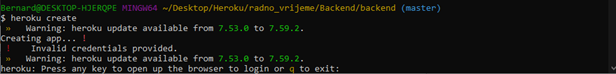
\includegraphics[width=\textwidth]{Dokumentacija/pogon/Picture2.png}
				\caption{Pokretanje Heroku u Git-u}
				\end{figure}
				Nakon što se upiše bilo koji znak u web pregledniku će nam se pojaviti ova stranica : 
				\begin{figure}[H] 					\centering 					                \includegraphics[width=\textwidth]{Dokumentacija/pogon/Picture3.png}
				\caption{Heroku web-stranica}
				\end{figure}
				Prije puštanja u pogon moramo namjestiti varijable za bazu podataka u application.properties. Datoteka se nalazi u .../backend/src/main/resources/ i treba izgledati kao sljedeće: 
				\begin{figure}[H] 					\centering 					                \includegraphics[width=\textwidth]{Dokumentacija/pogon/Picture4.png}
				\caption{Prikaz datoteke za varijable baze podataka}
				\end{figure}
				Mora se specificirati koju verziju jave koristimo u aplikaciji da Heroku zna kako ju pokrenuti. Url, korisničko ime i lozinku navodimo tako jer ih Heroku upisuje pomoću svojih varijabli okruženja. Koristi se također PostgereSQLDialect pošto heroku baze podataka stvara u Postgresql. 

Nakon podešavanja application.properties u bash upisujemo “git push heroku master” 
				\begin{figure}[H] 					\centering 					                \includegraphics[width=\textwidth]{Dokumentacija/pogon/Picture5.png}
				\caption{"git push heroku master" rezultati}
				\end{figure}
				Time smo završili sa puštanjem backend aplikacije u pogon. 

 

\textbf{Puštanje frontend aplikacije u pogon }

Postupak za frontend aplikaciju je skoro identičan kao i za backend aplikaciju. 

Prebacuje se u mapu \textit{.../radno\char`_vrijeme/frontend/ui} i tamo se treba otvoriti Git Bash. Inicijaliziramo novi git repozitorij pomoću naredbe “git init”. Dodajemo i commitamo sve datoteke u tom folderu naredbama “git add .” i “git commit -m “Prvi commit””.  

				\begin{figure}[H] 					\centering 					                \includegraphics[width=\textwidth]{Dokumentacija/pogon/Picture6.png}
				\caption{Prvi commit za frontend}
				\end{figure}
				Nakon toga upisujemo komandu “heroku create”. Pošto smo već ulogirani odma će stvoriti novu aplikaciju. 

Prije puštanja aplikacije u pogon moramo u .env dokumentu upisati lokaciju backend-a. 
				\begin{figure}[H] 					\centering 					                \includegraphics[width=\textwidth]{Dokumentacija/pogon/Picture7.png}
				\caption{Adreasa backend aplikacije}
				\end{figure}
				Ovdje se ime-aplikacije odnosi na to kako nam se na Heroku zovu aplikacije. 

Zadnji korak je staviti izvorni kod u tu aplikaciju što se radi pomoću komande heroku “git push heroku master”. 
				\begin{figure}[H] 					\centering 					                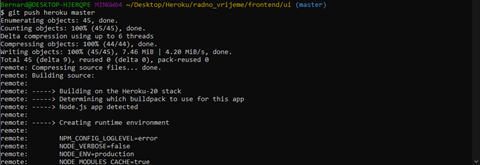
\includegraphics[width=\textwidth]{Dokumentacija/pogon/Picture8.png}
				\caption{"git push heroku master" za frontend}
				\end{figure}
				Ovime smo završili sa puštanjem frontend aplikacije u pogon. 

Aplikacije možemo vidjeti na svome profilu na Heroku i otvarati ih preko linkova “https://ime-aplikacije.herokuapp.com” 
				\begin{figure}[H] 					\centering 					                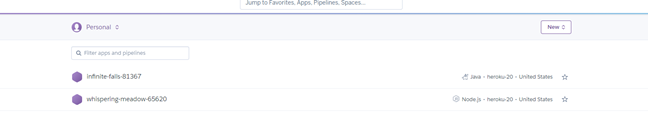
\includegraphics[width=\textwidth]{Dokumentacija/pogon/Picture9.png}
				\caption{Prikaz aplikacije na Heroku}
				\end{figure}
				
				

\textbf{Punjenje baze podataka} 

Baza podataka se automatski stvorila sa backend aplikacijom zbog definicija u application.properties.  
				\begin{figure}[H] 					\centering 					                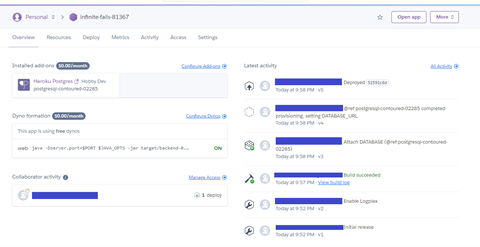
\includegraphics[width=\textwidth]{Dokumentacija/pogon/Picture10.png}
				\caption{Prikaz baze podataka uz backend aplikaciju}
				\end{figure}
				Do detalja baze dolazimo klikom na Heroku Postgres add-on i oni će nam trebati za postavljanje pristupa bazi. 
				\begin{figure}[H] 					\centering 					                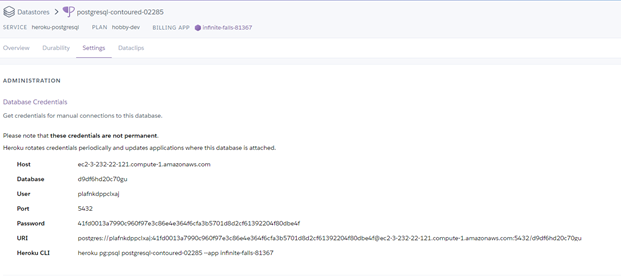
\includegraphics[width=\textwidth]{Dokumentacija/pogon/Picture11.png}
				\caption{Detalji baze podataka}
				\end{figure}
				Treba se instalirati pgAdmin na računalo pomoću windows installera koji možemo naći na službenoj stranici. 

Nakon što otvorimo aplikaciju prvi put potrebno je stvoriti korisničko ime i lozinku po volji. Sada se treba stvoriti nova veza na server gdje se nalazi baza. Server se naziva po volji i u polja upisujemo vrijednosti koje se nalaze u detaljima naše baze na Heroku.  
				\begin{figure}[H] 					\centering 					                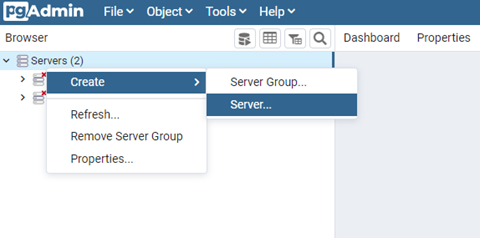
\includegraphics[width=\textwidth]{Dokumentacija/pogon/Picture12.png}
				\caption{pgAdmin stvaranje poslužitelja}
				\end{figure}
				 
				\begin{figure}[H] 					\centering 					                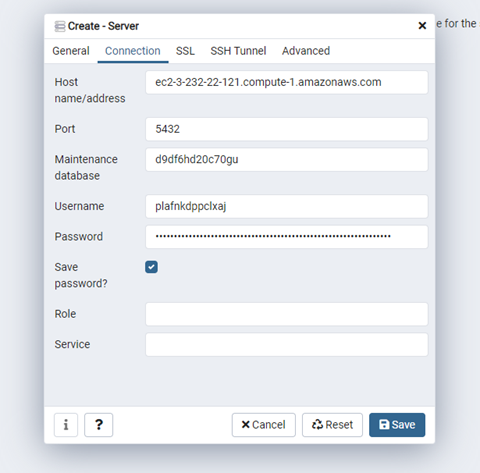
\includegraphics[width=\textwidth]{Dokumentacija/pogon/Picture13.png}
				\caption{pgAdmin4 stvaranje poslužitelja 2. dio}
				\end{figure}
				Sada među bazama podataka na HerokuServer nađemo našu i otvorimo Query Tool. U njemu otvorimo dokument \textit{partial\char`_database\char`_fill.sql} koji se nalazi u \textit{.../radno\char`_vrijeme/Database} i pokrenemo ga. Time smo napunili našu bazu podataka.
				\begin{figure}[H] 					\centering 					                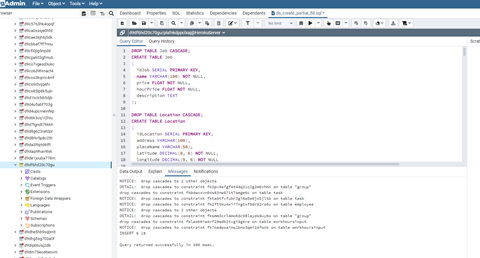
\includegraphics[width=\textwidth]{Dokumentacija/pogon/Picture14.png}
				\caption{pgAdmin4 "query tool"}
				\end{figure}
			
			
			\eject 